\chapter{Realization} \label{chapter:realization}
After having discussed the basic concept of the approach in the previous chapter, in this chapter, an exemplary realization is presented. Previously, three key challenges were identified:
\begin{inparaenum}[(i)]
  \item \emph{reliable, anonymous information exchange},
  \item \emph{isolation}, and
  \item \emph{connectivity} (\cf \ref{sec:challenges}). 
\end{inparaenum}
To tackle these challenges, three technologies are proposed:

\begin{enumerate}[(i)]
\item \textbf{DDS} to enable \emph{reliable, anonymous information exchange},
\item \textbf{\docker} as containerization tool to achieve \emph{isolation} and portability of services, and
\item \textbf{\wnet} as means to provide \emph{connectivity} between the containerized services.
\end{enumerate}

In the following, these three tools are presented and it is described how they were leveraged to realize the system.

\section{DDS for Data Exchange}

DDS is a promising candidate for a middleware that fulfills requirements to a satisfying degree.

OpenDDS was used.

Why DDS?

\paragraph{Versatile transport methods.} Supports shared memory (especially important), UDP and TCP transports

\paragraph{Dynamic Service Discovery.} Service discovery is extraordinarily fast and dynamic. Lost connections are picked up as soon as possible.

\paragraph{Data Centricity and Anonymous Messaging.}

\paragraph{Asynchronous Messaging.}

\paragraph{Location Transparency.}

\paragraph{Decentralization.}

\paragraph{Platform Independence.}


\subsection{Redundancy and Automatic Failover} \label{sec:failover}
DDS has ways to ensure reliable communication---even over unreliable transmission channels. Part of reliability is failure transparency, \ie , the ability to quickly substitute failed components by backup components. By means of certain DDS features, it is possible to realize such behavior. The substitution process involves two steps: first, the failure needs to be detected. Second, a backup service needs to be instructed to take over. Three QoS policies are needed to realize this process: \ownership , \ostrength\ and \liveliness\ (\cf \autoref{tab:qos}).

As the first step, a mechanism needs to determine whether a component has failed. In most cases, it is not possible for a failing component to properly shut down and "sign off", \ie , to notify the rest of the system that it will become unavailable. For this reason, the failure needs to be automatically registered. The \liveliness\ policy can be used to achieve this. \liveliness\ is the mechanism that determines whether a service is responsive ("alive"), or unresponsive ("dead"). The policy's value can be set to number indicating the maximum time interval between each liveliness signal. If a service fails to show a vital sign during that period, it is considered dead by the rest of the system. Passive components, \ie\ those which do not actively emit data, can be instructed to automatically send liveliness signals, or heartbeats, in certain intervals.

After a service has been declared dead it is up to the middleware to elect a substitute service. This is done through the \ownership\ and \ostrength\ QoS policies. By assigning a topic the \ownership\ value "\qos{exclusive}" one can specify that only a single data writer may write to that topic at any given time. Which data writer is given that prerogative is determined by the data writer's \ostrength\ value. The data writer that possesses the higher value is eligible to write to the topic. In the failover scenario, both, the primary service and the backup service are assigned to the same topic, and both are configured to have exclusive \ownership\ rights. The former one has a higher \ostrength\ than the latter one. Based on this value, the backup service can be instructed to take over.


\subsection{DDS for Automotive Systems}
Automotive software systems have previously relied -- and, to some degree, will continue to do so -- on low-level, low-bandwidth transport protocols such as CAN, LIN, etc. For the longest time, networks stacks based on those protocols were sufficient to meet the basic requirements of delivering vehicular sensor data and x-by-wire functions. However, driven by the emergence of innovative functions, the demands for vehicle intrinsic networks are skyrocketing. In particular, more and more sensor data from increasingly bandwidth-hungry sensors, such as cameras and LIDARs is feeding into advanced systems such as ADAS. At the same time, these functions require computational capabilities that go way beyond of what is possible with the microcontrollers typically used in traditional ECUs. High-performance computer systems based on high-level operating systems, supported by bandwidth-friendly networking protocols are needed to meet the new requirements. A new generation of low-level network protocols found their way into the vehicle. Notable mentions are FlexRay, and TSN. A question that remains is whether DDS is a suitable choice for the use within vehicles, and whether DDS may be used efficiently on top of these lower level protocols. \citeauthor*{bouhouch2013dds} have shown \cite{bouhouch2013dds} that DDS is indeed a suitable middleware to be used in vehicular networks.


DDS is designed for resource constrained real-time applications such as sensor networks or industrial automation.

DDS allows to configure how much of a system's resources an DDS-enabled application may use. Consequently, it is the middleware's responsibility to allocate resources as needed while still staying within the specified boundaries. At the same time, priorities aligning with the application's QoS settings need to be considered. DDS takes this burden off the programmer's shoulders.



\subsection{Separation of User Data}
\todo[inline]{nur eine idee}
The presented approach relies on a single cloud infrastructure, while at the same time, a vast number of customers need to be served. This poses a challenge concerning the separation of data. Confidentiality and privacy of user-specific application data must be preserved. Similarly, the result of a computation commissioned by a specific vehicle must be returned to exactly that vehicle, and no one else. 

Gladly, DDS offers a solution to this. In DDS, topics are not restricted to a single domain, \ie , they may be reused in multiple domains. If, \eg , a publisher belongs to \texttt{Domain $\alpha$} and publishes data on \texttt{Topic A}. Then, a data reader that reads from \texttt{Topic A} but belongs to \texttt{Domain $\beta$} may not read the data. Therefore, through domains, the same application may be reused several times, while keeping topic data separate. This principle is take advantage of in the presented approach: Domains are used to separate user data, such that for each user there is one user-specific domain.

%
%
%
%
%
%
%
%
%
%

\section{\docker\ for Containerization}

\todo[inline]{todo}
\begin{itemize}
	\item Portability: Containers need to run in vehicles and cloud -> \docker is available on many platforms, ARM version is fully functional
Besides providing isolation, \docker\ has a number of other benefits.
	\item Innovation Pressure: not docker specific) calls for fast development cycles -> CI/CD.
	\item light-weight: Important for embedded systems, provides: fast spin-up, low overhead
\end{itemize}


\docker\ is a holistic containerization platform which includes everything needed to build, run, deploy, and distribute containers. The \docker\ application is structured in a client-server model (\cf \autoref{fig:docker-arch}). The server is a daemon process running at all times on the host machine. Its primary purpose is to manage containers, images, networks and data volumes, and to provide the means to  build images and run containers. The \docker\ server exposes a RESTful HTTP API by which it can be controlled. The client side of the \docker\ application is a command line interface (CLI) which acts as a user friendly façade for the server's API.

\begin{figure}[htpb]
  \centering
  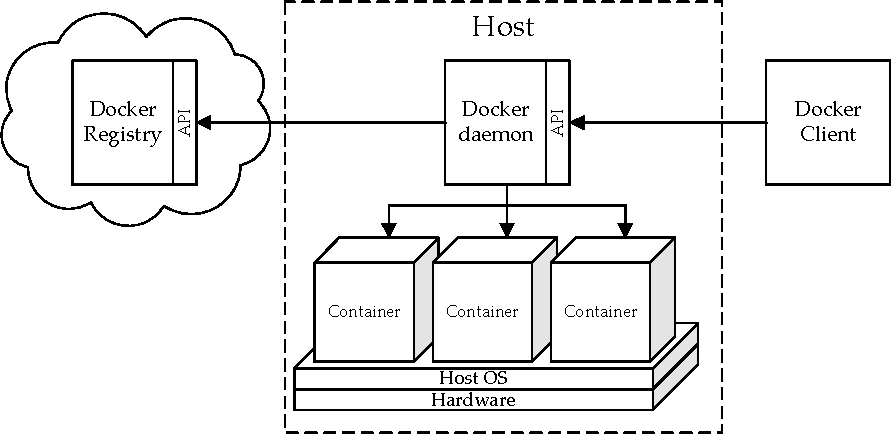
\includegraphics[width=0.8\textwidth]{figures/docker-arch.pdf}
  \caption[\docker\ architecture]{\docker\ architecture}\label{fig:docker-arch}
\end{figure}

\subsection{\docker\ Components}
Container images may be seen as the "blueprint" on the basis of which containers are built. They define exactly which files and directories are contained in a container once it comes to life. Effectively, every container is an instantiation of an image of a certain type, in the same way an object is an instantiation of a class in an object-oriented programming language. While the concept of images is very common among containerization and virtualization tools, \docker\ follows a rather unconventional approach. In \docker , images are made up of series of read-only file system layers. Each layer may add files and directories to its respective underlying layer. If a layer tries to modify a file from an underlying layer it creates a copy of that file and adds it to its own layer. The modification is then performed on the copy instead of the original. This principle called "Copy on Write" (CoW) ensures that layers cannot be modified which makes it possible to share individual layers with other images stored on the host. By treating images as a collection of individual, sharable pieces instead of atomic units, massive storage space savings can be achieved. Another benefit of this is that whenever a container is started, only a thin writable layer needs to be added on top of an image, and the underlying layers do not need to be copied. That way, start-up times of containers are kept extremely low. \todo{how low? quellen} Virtual Machines, in contrast, would first need to boot into an operating system prior to operation.
\paragraph{}
\docker\ images are defined in so-called \emph{Dockerfiles}. Dockerfiles are made up of series of instructions that tell \docker\ how to build a certain image. Each instruction adds another file system layer to the image. An example of a Dockerfile is depicted in \autoref{lst:dockerfile}. The first line defines the base image on top of which this particular image shall be built. In this case, an image called "debian" was chosen. As the name suggests, that base image contains a basic installation of the Linux distribution Debian\footnote{\url{www.debian.org}}. Next, the line \ \texttt{COPY . /application} \ instructs \docker\ to copy the contents of the current (host) directory to the image's \ \texttt{/application} \ directory. The changes in the file system are added in the form of a layer---the underlying layers are not affected. The \ \texttt{RUN} \ instruction in the following line causes \docker\ to run the subsequent commands within the container. In this case, the newly added application directory is entered and the command \ \texttt{make} \ is executed, effectively compiling the application. Again, the resulting changes to the file system are encapsulated within another layer. In practice, the now topmost layer would contain all files produced by \ \texttt{make}. Finally, the \ \texttt{ENTRYPOINT} \ instruction defines the action to be performed once the container is started. In this case, the shell script \ \texttt{run.sh} \ would be executed within the container. This command, too, would add a layer to the image, albeit an empty one. By defining images as sequences of instructions, reproducibility is guaranteed.
\begin{lstlisting}[caption=An examplary Dockerfile, label=lst:dockerfile, numbers=left, numberstyle=\tiny]
FROM debian
COPY . /application
RUN cd /application && make
ENTRYPOINT /application/run.sh
\end{lstlisting}
By running the command \ \mbox{\texttt{docker build -t IMAGENAME .}} \ in the directory of the Dockerfile, an image based on that Dockerfile would be built. Using the command \ \texttt{docker run IMAGENAME}, a new container of that image type would be launched.



\paragraph{}
\docker\ images may be stored in \emph{\docker\ Registries}, where they can be browsed, managed, and distributed. The command \ \texttt{docker push IMAGENAME[:TAG]} \ causes the image with the name \ \texttt{IMAGENAME} \ to be uploaded to a registry. Analogously, to download an image from a registry, one would have to run the command \ \texttt{docker pull IMAGENAME[:TAG]}. \docker\ registries are implemented as a server software which exposes an HTTP API. The registry server is open source\footnote{\url{www.github.com/docker/distribution}} and may be deployed on any server that supports it. The \docker\ company itself hosts one of such registries, Docker Hub\footnote{\url{hub.docker.com}}, which is provided as a publicly available  and free-to-use service. 

\subsection{\docker\ Engine}
The engine takes a container image and turns it into a container, \ie , a running process.



\subsection{Multi Platform Compatibility} \label{sec:multiplat}
The primary purpose of containerization is to provide portable execution environments that allow software to run on a broad range of computing systems. A limitation of containers is that they only provide portability across \emph{operating systems}, and not \emph{hardware platforms}. In other words, containers do not provide binary compatibility. The reason for this is that containerized applications run directly on the kernel of the host system, and do not build on top of a virtualization layer as classic VMs do. As a result, a containerized binary built for an x86-based processor will not run on an ARM system, and vice versa. This is problematic especially in the context of embedded systems which often rely on particular hardware architectures that favor energy efficiency over performance. Computing nodes in a data centers, on the other hand, are typically based on architectures aimed at providing a maximum level of performance. As the presented approach intends containers to be deployed on both, vehicular on-board systems and in the cloud, this poses a challenge. 

Several approaches exist to tackle this problem. For example, one could embed a thin platform compatibility layer at the base of each container. This approach was popularized by \emph{resin.io}\footnote{\url{www.resin.io}}. resin.io is a company that specializes in containerization for IoT devices. On their Docker Hub page\footnote{\url{hub.docker.com/u/resin}} they provide \docker\ images which have the \emph{QEMU}\footnote{\url{www.qemu.org}} machine emulator built in. Facilitated by QEMU's user emulation mode, binaries built for a given processor architecture may be executed on otherwise incompatible processors. QEMU achieves this by translating any guest system calls into host system calls. The previously mentioned images are built in a way that allows any arbitrary binary executed within such container to be run in the context of QEMU. Thus, the container may run on a multitude of hardware platforms.
This approach simplifies the software build process tremendously as only one container per service needs to be built. This container can then be reused for all platforms. However, this way of achieving multi-platform portability turned out to be unsuitable for the intended use case as multicast is not well supported by QEMU. 

Thus, another approach was leveraged to solve the multi-platform compatibility issue. This approach builds on Continuous Integration (CI) in accord with Docker Hub, and in particular, Docker Hub's \emph{image manifest} feature. By default, a \docker\ image name corresponds to exactly one image. Thus, whenever an image with a given name is requested from the \docker\ registry, only that specific image is returned to the requester. Image manifests extend registries by the option to define \emph{multiple} images per image name. That way, several containers, each specifically built for a given platform, may be deployed under the same name. Depending on the requesting node's hardware architecture, a different image may be returned. \autoref{fig:manifest-pull} depicts an example for this. In the example, an x86-based machine requests the \texttt{some/image:v1.0} image from the registry. What is then returned from the registry is an image specifically made for x86 architectures. On the other hand, an ARM-based machine which requests the very same image, \texttt{some/image:v1.0}, receives an entirely different image as a response. This kind of behavior is achieved through an image look-up in the manifest file which is performed behind the scenes. 

\todo[inline]{Bilder: docker repository -> docker registry}

\begin{figure}[htpb]
  \centering
  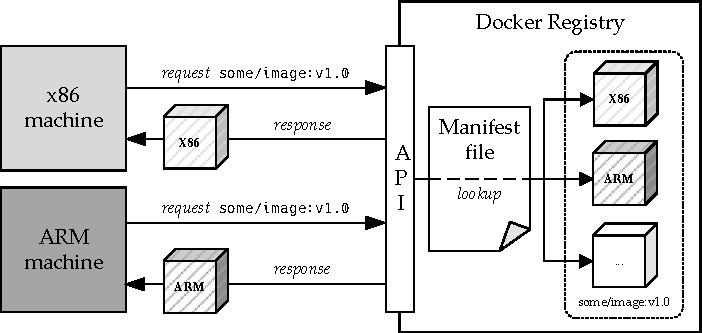
\includegraphics[width=0.8\textwidth]{figures/manifest-pull}
  \caption[Pulling \docker\ images via manifest file]{Two nodes request the same image name but receive different images which are specifically built for their respective processor architecture. Which node requires which image is determined by a look-up in the manifest file.}\label{fig:manifest-pull} 
\end{figure}

A disadvantage of this approach (compared to the QEMU one) is that multiple versions of the same container need to be built every time a service receives a software update. To cope with this hindrance, a minimal CI pipeline was leveraged. Consider \autoref{fig:manifest-push} in which the employed service deployment process is depicted. The build process is initiated whenever a code change is pushed to the remote git repository. Once a push is registered, the CI Platform (Travis CI\footnote{\url{www.travis-ci.org}} was used) pulls the latest version from the git repository and executes a build script. The build script compiles several version of the service for each target platform, embeds the binaries in images and pushes those images to the \docker\ registry (Docker Hub).

\begin{figure}[htpb]
  \centering
  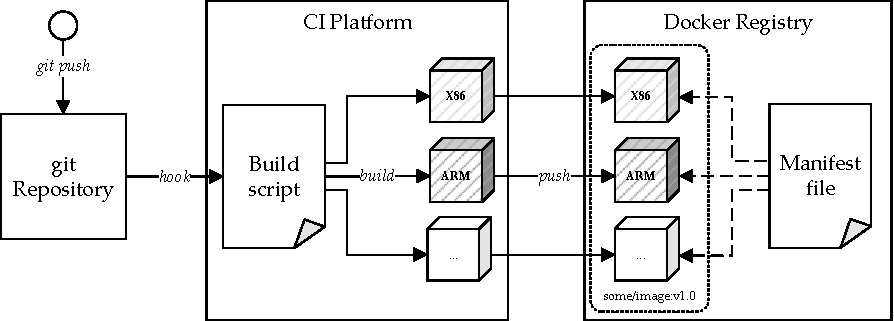
\includegraphics[width=\textwidth]{figures/manifest-push}
  \caption[Pushing \docker\ images via CI]{A git push to a service's git repository triggers the build process in the CI platform: the code is compiled for several platforms and the resulting images are pushed to the \docker\ registry.}\label{fig:manifest-push} 
\end{figure}

%
%
%
%
%
%
%
%
%
%
%
\subsection{Containerized Services}
In the envisaged system, each service is packed into its own container with all its dependencies. That way, services may run wherever they are placed, and thus, a great deal of portability is achieved. \docker 's layered approach to images is immensely helpful in this.\todo{???}
\begin{figure}[htpb]
  \centering
  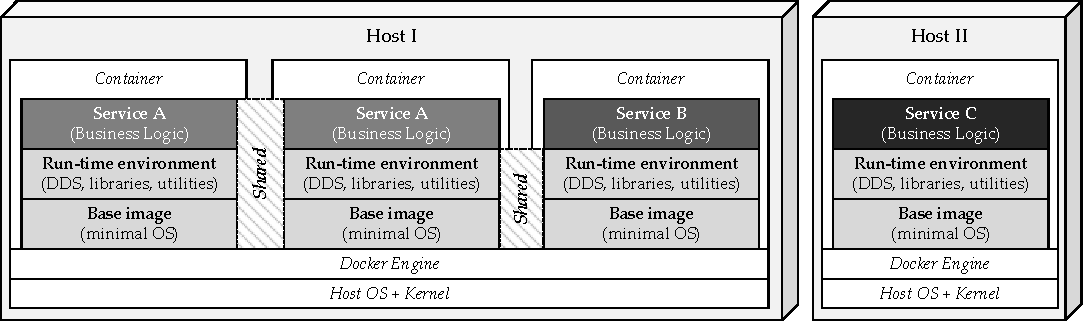
\includegraphics[width=\textwidth]{figures/docker-sharing}
  \caption[An example of containerized services]{An example of four containerized service instances, some sharing common logic to save disk space and facilitate fast updates}\label{fig:service-containers} 
\end{figure}
\autoref{fig:service-containers} shows an example of three containerized services running on two different machines, \experim{Host I} and \experim{Host II}. On the former, two instances of \experim{Service A}, and one instance of \experim{Service B} are placed. On the second host only one service instance is deployed, namely one of type \experim{Service C}. All services are packaged in their own, separate container. The containers are made up of three stacked images---the bottom two are common to all services. The bottommost image ("\emph{base image}") contains the file system layers of a minimal operating system. In this thesis, the Linux distribution Debian was used. The base image only contains a limited selection of Linux tools, such as \ \texttt{ls}, \texttt{cat}, \texttt{ps} \ etc. The purpose of a base image is to lay a solid foundation that enables users to work comfortably within the container. In the case of Debian, the \emph{aptitude} package manager is additionally included which enables users to easily install further tools. 

Next, an \emph{intermediate image} is built on top of the base image. The intermediate image adds further layers containing the \emph{run-time environment}, and in particular, the shared libraries of OpenDDS. This image could optionally contain more libraries and tools that are common to all services. For the purpose of demonstration, however, DDS is sufficient\todo{updaten, falls es zu case study kommt} . The base image and the intermediate image lay the foundation of all services. Any image built on top of these could run an DDS-enabled service. \docker 's layered images allows these layers to be shared \todo{besser erklaeren}

At the top, finally, sit the \emph{service images}. In these images contained is the actual service logic, and more precisely, the service's binary and configuration files. The service images are unique to each service, and are not shared, except when the same service is instantiated multiple times on the same machine (\cf \experim{Service A} in \autoref{fig:service-containers}).



\section{Container Networking with \wnet}
\wnet\ is an open source project\footnote{\url{www.github.com/weaveworks/weave}} which is developed by a global team, mostly employed by the London-based software company \emph{Weaveworks}\footnote{\url{www.weave.works}}. The purpose of \wnet\ is to provide advanced overlay networking capabilities for \docker\ containers. As such, is designed to make up for the shortcomings of \docker 's built-in overlay networks, and more specifically, their lack of encryption and multicast support. By means of \weave\ overlay networks, dispersed containers deployed on physically isolated hosts around the world, may communicate as if they were connected via LAN. From a containerized applications' viewpoint, it does not matter whether its peers are located on the same host or within a data center on the other side of the world. 

\paragraph{}

\wnet\ is implemented as client software which is installed on each machine that partakes in the overlay. The software can be started using a single command, and in the following, all containers launched on that host will automatically connected to the overlay network. This is achieved by means of a \emph{\docker\ API proxy}. The proxy sits between \docker 's command-line client and the \docker\ daemon and intercepts all communication between the two. When the \docker\ engine is instructed to start a container, the proxy takes all precautions needed to enable overlay networking for that container. Once the connection is established, all container traffic is routed through three dedicated network channels: one TCP connection to exchange meta data about the network, and two UDP channels for duplex data exchange.

\begin{figure}[htpb]
  \centering
  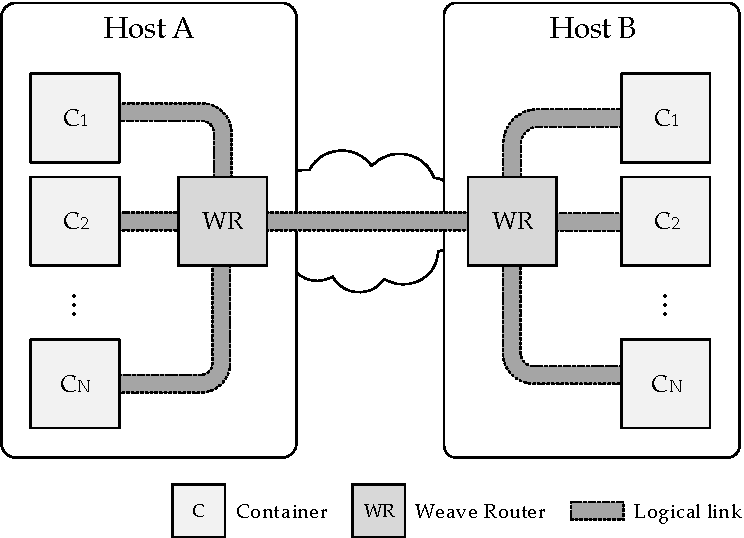
\includegraphics[width=0.7\textwidth]{figures/weave.pdf}
  \caption[An example of containers connected via \wnet\ overlay network]{A number of dispersed containers connected by a \wnet\ overlay network}\label{fig:weavescheme} 
\end{figure}

When the \weave\ software is started, a central component of \wnet , the \emph{\weave\ router} is launched (\cf\ \autoref{fig:weavescheme}). Similar to a hardware router, the \weave\ router is responsible for the forwarding and routing of data packets to their appropriate receivers. \weave\ routers can be seen as gateways through which all containers participating in a \weave\ network are connected. To facilitate routing on the data plane, a custom UDP encapsulation protocol, called \emph{sleeve}, was devised. A \weave\ router in itself is an containerized application running at all times, in the same way a daemon would. There is one of such router containers running on every host in a \weave -enabled infrastructure.

\todo[inline]{ÜBERARBEITEN}

The \weave\ router is a user space process. As such, a context switch is needed every time it is tasked to process a packet. This comes with a substantial performance overhead. Hence, as a faster alternative, the so-called \emph{fast datapath} mode was added. In this mode, packets are processed by the Linux kernel instead of by the \weave\ router. This way, the context switch into user space is omitted. \wnet\ leverages the Linux kernel's \emph{Open vSwitch datapath} module \cite{pfaff2015design} to achieve this behavior. Open vSwitch can be used to create a virtual, software-based network switch. That way, the kernel can be instructed to process packets in a certain way. For instance, the kernel can be commanded to add a VXLAN header to each packet, thereby achieving the same result as the \weave\ router, but faster. However, fast datapath mode can only be used when the underlying infrastructure allows it. The Internet is a particular example of a network where fast datapath communication is hard to achieve.


\subsection{Topology Management} 
\weave 's topology management is self-governing and self-healing. Peers continually exchange topology information and monitor the state of the network. Whenever peers lose connectivity, they continuously try to re-establish the connection until it is restored. All participating peers know the topology of the entire network. For this, \wnet\ employs a sophisticated discovery and topology management mechanism by which changes in the network topology are rapidly propagated within the network. The topology management protocol is based on a spanning-tree broadcast mechanism known from hardware switches. To further ensure that all peers have an up-to-date neighbor list at all times, \wnet\ additionally employs a custom neighbor gossiping protocol by which each peer sends update messages to a random subset of their neighbors. Updates of the network's topology are performed periodically as well as when certain events occur, such as when a node joins or leaves the network.

In order to add a new host to the overlay, the \weave\ software needs to be started on that host, referencing at least one other host in the network by its IP address. The information that a new host was added is then propagated to the other hosts in the overlay. After a short period, all hosts know that the new host was added and that a path to that host exists.

\subsection{Encryption} 
As mentioned earlier, a salient feature of \wnet\ is the ability to encrypt all traffic within the overlay network\footnote{Encryption applies end-to-end between \weave\ routers}. This is especially important for networks that span over insecure underlays, such as the Internet. To set up encryption, a shared secret (password) needs to be provided when the \weave\ router is launched. The shared secret must therefore be present on all participating hosts. From the password, salted, ephemeral session keys are generated which are then used to encrypt the network packets' payload. For each connection between any two peers, one unique session key exists.

The way encryption is applied differs depending on the forwarding mode used (sleeve or fast datapath). In fast datapath mode, a IPsec-based protocol is used, whereby each packet is wrapped in an encapsulated security payload (ESP). Because each packet in this mode is processed by the Linux kernel, encryption is applied by means of the standard Linux Kernel Crypto API which is thoroughly tested, and generally considered secure. For sleeve mode, a custom encryption algorithm based on TLS\footnote{``Transport Layer Security''} is used. As with fast datapath encryption, sleeve mode encryption utilizes shared, ephemeral session keys for each connection.

\begin{figure}[htpb]
  \centering
  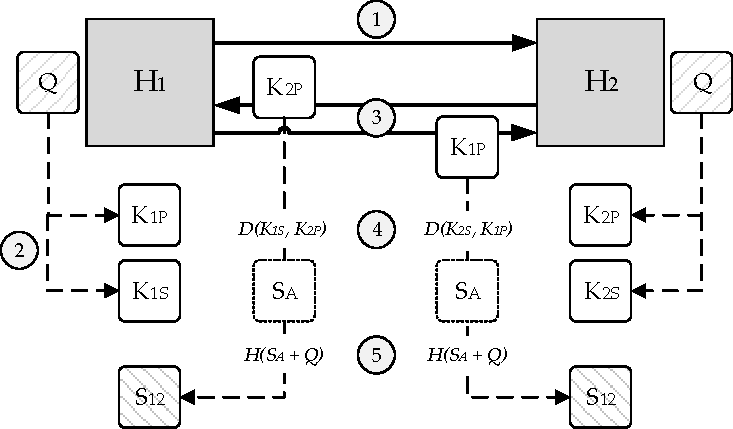
\includegraphics[width=0.6\textwidth]{figures/weave-encryption.pdf}
  \caption[\weave 's key exchange protocol]{\wnet 's key exchange protocol in sleeve mode}\label{fig:weaveencryption}
\end{figure} 
\autoref{fig:weaveencryption} depicts how these session keys are generated. In the image, two hosts ($H_1$, $H_2$) are to establish an encrypted connection. First, $H_1$ initiates the key exchange by sending a handshake message to $H_2$ \circled{1}. Then, both hosts generate their own, individual key pairs so that each host has a public key and a private key \circled{2}. The key pair for $H_1$ is $(K_{1P}, K_{1S})$ and the key pair for $H_2$ is $(K_{2P}, K_{2S})$. Once that is done, both hosts exchange their respective public keys, $K_{1P}$, and $K_{2P}$ \circled{3}. Using the peer's public key and their own private key, both hosts derive an auxiliary shared key, $S_A$, by means of Diffie--Hellman key exchange \cite{bresson2001provably}: $D(K_{1S},K_{2P})$ \circled{4}. Finally, the actual shared key can be generated. For this, both hosts append the password ($P$) to $S_A$ to provide authenticity. In order to bring the key to the desired length of 256 bit, the compounded key is additionally hashed via SHA256: $H(S_A, P)$ \circled{5}. The end result of this procedure is the final shared key, $S_{12}$, which is then used to encrypt the traffic between the two hosts.
%
%
%
%
%
%
%
%
%
%
%
%
%
%
%
%
%
%
%
%








